% =====================================================================
%  5.5 Sammensatte problemer — teori og oppgaver
% =====================================================================

\del{1}{Teoretiske problemer}

\begin{ordliste}
diagonal & En rett linje mellom to hjørner i en mangekant som ikke er naboer. & \mittsprak\\
regulær mangekant & En mangekant der alle sidene er like lange og alle vinklene er like store. & \mittsprak\\
sentralvinkel & Vinkelen ved sentrum $O$ mellom to nabohjørner i en regulær mangekant. & \mittsprak\\
strategi & En plan i flere steg som du kan bruke på mange oppgaver. & \mittsprak\\
eksakt svar & Et svar uten avrunding, for eksempel $4\sqrt3 + 6$. & \mittsprak\\
\end{ordliste}

\begin{mustkunne}
\begin{minipage}[t]{0.50\linewidth}
\textbf{Strategi i fem punkter}
\begin{enumerate}[leftmargin=1.4em,itemsep=1pt,topsep=2pt]
  \item \textbf{Tegn og merk.} Sett inn alt som er kjent. Merk det du skal finne med ?.
  \item \textbf{Finn en trekant} der du kjenner nok til å bruke en setning.
  \item \textbf{Regn ut} det du trenger videre.
  \item \textbf{Gå til neste trekant} og bruk det du fant.
  \item \textbf{Kontroller:} vinkelsum $180^\circ$, og den lengste siden ligger overfor den største vinkelen.
\end{enumerate}
\end{minipage}\hfill
\begin{minipage}[t]{0.47\linewidth}
\textbf{Hva er kjent? Hvilken setning?}\par
\renewcommand{\arraystretch}{1.3}
\begin{tabular}[t]{@{}>{\raggedright\arraybackslash}p{3.7cm} >{\raggedright\arraybackslash}p{3.4cm}@{}}
rett vinkel & $\sin$, $\cos$, $\tan$, Pytagoras\\
vinkel og siden overfor, pluss én til & sinussetningen\\
to sider og vinkelen mellom, eller tre sider & cosinussetningen\\
to sider og vinkelen mellom, areal & arealsetningen\\
\end{tabular}
\end{minipage}
\par\smallskip
\textbf{Hvorfor flere trekanter?} Ofte har ingen trekant nok opplysninger alene. Da bruker vi en side eller vinkel som to trekanter deler (for eksempel en diagonal). Den første trekanten gir den manglende opplysningen til den neste.
\end{mustkunne}

\begin{eksempel}[1 — firkant med diagonal]
\begin{minipage}[t]{0.52\linewidth}I firkanten $ABCD$ er $AB = AD = 4$, $\angle A = 60^\circ$, $BC = 3$ og $\angle DBC = 90^\circ$. Finn diagonalen $BD$, siden $CD$ og arealet av firkanten. Svar eksakt.
\end{minipage}\hfill
\begin{minipage}[t]{0.45\linewidth}
\centering
\begin{tikzpicture}[baseline=(current bounding box.north),scale=0.6,font=\small]
  \coordinate (A) at (0,0);
  \coordinate (B) at (4,0);
  \coordinate (D) at (2,3.464);
  \coordinate (C) at (6.598,1.5);
  \draw[thick] (A)--(B) node[midway,below] {$4$};
  \draw[thick] (B)--(C) node[midway,below,sloped] {$3$};
  \draw[thick] (D)--(C);
  \draw[thick] (A)--(D) node[midway,above,sloped] {$4$};
  \draw[dashed] (B)--(D) node[midway,right] {\color{niv3}\bfseries ?};
  \draw (3.85,0.26)--(4.11,0.41)--(4.26,0.15);
  \draw (0.7,0) arc (0:60:0.7);
  \node[font=\scriptsize] at (1.15,0.3) {$60^\circ$};
  \node[below left] at (A) {$A$};
  \node[below right] at (B) {$B$};
  \node[right] at (C) {$C$};
  \node[above] at (D) {$D$};
\end{tikzpicture}
\end{minipage}

\smallskip
\begin{stegtabell}
$BD^2 = 4^2 + 4^2 - 2 \cdot 4 \cdot 4 \cdot \cos 60^\circ = 16$ & Trekant $ABD$ har to sider og vinkelen mellom: cosinussetningen.\\
$BD = 4$ & Ta kvadratroten. (Trekanten er likesidet.)\\
$CD^2 = 4^2 + 3^2 = 25$, så $CD = 5$ & Trekant $BCD$ er rettvinklet i $B$: Pytagoras.\\
$T_{ABD} = \frac12 \cdot 4 \cdot 4 \cdot \sin 60^\circ = 4\sqrt3$ & Arealsetningen i $ABD$.\\
$T_{BCD} = \frac12 \cdot 4 \cdot 3 = 6$ & Rettvinklet: halvparten av katetene ganget.\\
$T = 4\sqrt3 + 6$ & Legg sammen de to trekantene.\\
Kontroll: & $ABD$ har $AB = AD$ og $60^\circ$ i toppen, så alle vinkler er $60^\circ$ og $BD = 4$. Det stemmer.\\
\end{stegtabell}
\end{eksempel}

\begin{eksempel}[2 — høyde i en trekant]
\begin{minipage}[t]{0.52\linewidth}I trekant $ABC$ er $\angle B = 45^\circ$, $\angle C = 30^\circ$ og $BC = 2 + 2\sqrt3$. Linja $AD$ er høyden fra $A$. Finn $h = AD$ og arealet.
\end{minipage}\hfill
\begin{minipage}[t]{0.45\linewidth}
\centering
\begin{tikzpicture}[baseline=(current bounding box.north),scale=0.8,font=\small]
  \coordinate (B) at (0,0);
  \coordinate (D) at (2,0);
  \coordinate (C) at (5.464,0);
  \coordinate (A) at (2,2);
  \draw[thick] (B)--(C)--(A)--cycle;
  \draw[dashed] (A)--(D) node[midway,left] {\color{niv3}\bfseries ?};
  \draw (1.8,0)--(1.8,0.2)--(2,0.2);
  \draw (0.5,0) arc (0:45:0.5);
  \node[font=\scriptsize] at (0.8,0.2) {$45^\circ$};
  \draw (4.764,0) arc (180:150:0.7);
  \node[font=\scriptsize] at (4.2,0.17) {$30^\circ$};
  \draw[|-|] (0,-0.65)--(5.464,-0.65) node[midway,below] {\scriptsize$2+2\sqrt3$};
  \node[left] at (B) {$B$};
  \node[right] at (C) {$C$};
  \node[above] at (A) {$A$};
  \node[below,yshift=-2pt] at (D) {\scriptsize$D$};
\end{tikzpicture}
\end{minipage}

\smallskip
\begin{stegtabell}
$BD = \dfrac{h}{\tan 45^\circ} = h$ & Rettvinklet $ABD$: $\tan 45^\circ = \frac{h}{BD}$ og $\tan 45^\circ = 1$.\\
$DC = \dfrac{h}{\tan 30^\circ} = \sqrt3\,h$ & Rettvinklet $ADC$: $\tan 30^\circ = \frac{1}{\sqrt3}$.\\
$h + \sqrt3\,h = 2 + 2\sqrt3$ & $BD + DC = BC$. Begge trekantene deler $h$.\\
$h(1 + \sqrt3) = 2(1 + \sqrt3)$, så $h = 2$ & Faktoriser og del på $1 + \sqrt3$.\\
$T = \frac12 \cdot (2 + 2\sqrt3) \cdot 2 = 2 + 2\sqrt3$ & Grunnlinje ganger høyde delt på to.\\
Kontroll: & $BD = 2$ og $DC = 2\sqrt3$. Summen er $BC$.\\
\end{stegtabell}
\end{eksempel}

\begin{vanligfeil}
\begin{itemize}[leftmargin=1.2em,itemsep=1pt,topsep=0pt]
  \item $\sin v = \frac{\text{motstående}}{\text{hypotenus}}$ gjelder ikke generelt i en trekant uten rett vinkel. I en likesidet trekant er alle sider like, så brøken ville blitt $1$, men $\sin 60^\circ = \frac{\sqrt3}{2}$.
  \item Du bruker en vinkel fra feil trekant. Ligger $D$ på $BC$ og $\angle ADB = 60^\circ$, er $\angle ADC = 180^\circ - 60^\circ = 120^\circ$, ikke $60^\circ$.
  \item Sinussetningen på en trekant med to sider og vinkelen mellom (SVS) er feil. Da har du ikke en vinkel og siden overfor. Bruk cosinussetningen.
\end{itemize}
\end{vanligfeil}

\nivaahode{1}

\oppg{1.1}{1}{\uh}
Hva er kjent? Velg setningen du vil bruke først: sinussetningen, cosinussetningen eller arealsetningen. Du skal ikke regne ut.
\begin{tasks}(2)
  \task $A = 40^\circ$, $B = 65^\circ$ og $a = 6$. Finn $b$.
  \task $b = 5$, $c = 9$ og $A = 50^\circ$. Finn $a$.
  \task $a = 4$, $b = 6$ og $c = 8$. Finn $C$.
  \task $a = 7$, $b = 3$ og $C = 30^\circ$. Finn arealet.
\end{tasks}

\oppg{1.2}{1}{\uh}
\begin{minipage}[t]{0.58\linewidth}
Linja $AD$ står vinkelrett på $BC$. Fullfør.
\begin{tasks}(1)
  \task Trekant $ABD$: $AD = AB \cdot \sin\skrivlinje[1cm] = 6 \cdot \skrivlinje[1cm] = \skrivlinje[15mm]$.
  \task Trekant $ADC$: $AC = \dfrac{AD}{\sin\skrivlinje[1cm]} = \skrivlinje[2cm]$.
\end{tasks}
\end{minipage}\hfill
\begin{minipage}[t]{0.38\linewidth}
\centering
\begin{tikzpicture}[baseline=(current bounding box.north),scale=0.5,font=\small]
  \coordinate (B) at (0,0);
  \coordinate (A) at (3,5.196);
  \coordinate (D) at (3,0);
  \coordinate (C) at (8.196,0);
  \draw[thick] (B)--(C);
  \draw[thick] (B)--(A) node[midway,above,sloped] {$6$};
  \draw[thick] (A)--(C);
  \draw[dashed] (A)--(D) node[midway,left] {\color{niv3}\bfseries ?};
  \draw (2.7,0)--(2.7,0.3)--(3,0.3);
  \draw (1,0) arc (0:60:1);
  \node[font=\scriptsize] at (1.5,0.45) {$60^\circ$};
  \draw (6.7,0) arc (180:135:1.5);
  \node[font=\scriptsize] at (6.2,0.4) {$45^\circ$};
  \node[left] at (B) {$B$};
  \node[right] at (C) {$C$};
  \node[above] at (A) {$A$};
  \node[below] at (D) {$D$};
\end{tikzpicture}
\end{minipage}

\oppg{1.3}{1}{\uh}
\begin{tasks}(1)
  \task Hva er sentralvinkelen i en regulær sekskant, åttekant og tolvkant?
  \task I en regulær åttekant er $A$ og $B$ nabohjørner, og $O$ er sentrum. Finn vinklene ved $A$ og $B$ i trekant $OAB$. Forklar hvorfor trekanten er likebeint.
\end{tasks}

\nivaahode{2}

\oppg{1.4}{2}{\uh}
\begin{minipage}[t]{0.58\linewidth}
I firkanten $ABCD$ er $AB = 8$, $BC = 15$, $\angle B = 60^\circ$, $CD = 5$ og $DA = 12$.
\begin{tasks}(1)
  \task Finn diagonalen $AC$.
  \task Vis at $\angle D = 90^\circ$.
  \task Finn arealet av firkanten. Svar eksakt.
\end{tasks}
\end{minipage}\hfill
\begin{minipage}[t]{0.38\linewidth}
\centering
\begin{tikzpicture}[baseline=(current bounding box.north),scale=0.3,font=\small]
  \coordinate (B) at (0,0);
  \coordinate (A) at (8,0);
  \coordinate (C) at (7.5,12.99);
  \coordinate (D) at (12.19,11.25);
  \draw[thick] (B)--(A) node[midway,below] {$8$};
  \draw[thick] (B)--(C) node[midway,above,sloped] {$15$};
  \draw[thick] (C)--(D) node[midway,above,sloped] {$5$};
  \draw[thick] (A)--(D) node[midway,right] {$12$};
  \draw[dashed] (A)--(C) node[midway,left] {\color{niv3}\bfseries ?};
  \draw (2,0) arc (0:60:2);
  \node[font=\scriptsize] at (3.4,1.1) {$60^\circ$};
  \node[below left] at (B) {$B$};
  \node[below right] at (A) {$A$};
  \node[above] at (C) {$C$};
  \node[right] at (D) {$D$};
\end{tikzpicture}
\end{minipage}

\oppg{1.5}{2}{\uh}
\begin{minipage}[t]{0.55\linewidth}
Punktet $D$ ligger på $BC$ i trekant $ABC$. Vi vet at $AB = 6$, $\angle B = 45^\circ$, $\angle ADB = 60^\circ$ og $\angle C = 30^\circ$.
\begin{tasks}(1)
  \task Finn $AD$.
  \task Finn $AC$.
  \task Finn arealet av trekant $ADC$.
\end{tasks}
Svar eksakt.
\end{minipage}\hfill
\begin{minipage}[t]{0.41\linewidth}
\centering
\begin{tikzpicture}[baseline=(current bounding box.north),scale=0.45,font=\small]
  \coordinate (B) at (0,0);
  \coordinate (A) at (4.243,4.243);
  \coordinate (D) at (6.692,0);
  \coordinate (C) at (11.59,0);
  \draw[thick] (B)--(C);
  \draw[thick] (B)--(A) node[midway,above,sloped] {$6$};
  \draw[thick] (A)--(C) node[midway,above,sloped] {\color{niv3}\bfseries ?};
  \draw[thick] (A)--(D) node[midway,right] {\color{niv3}\bfseries ?};
  \draw (1.2,0) arc (0:45:1.2);
  \node[font=\scriptsize] at (1.9,0.4) {$45^\circ$};
  \draw (6.092,0) arc (180:120:0.6);
  \node[font=\scriptsize] at (5.2,0.55) {$60^\circ$};
  \draw (9.9,0) arc (180:150:1.7);
  \node[font=\scriptsize] at (9.2,0.45) {$30^\circ$};
  \node[left] at (B) {$B$};
  \node[right] at (C) {$C$};
  \node[above] at (A) {$A$};
  \node[below] at (D) {$D$};
\end{tikzpicture}
\end{minipage}

\oppg{1.6}{2}{\mh}
En regulær femkant har side $4,0$ cm. Sentrum er $O$. Tegn en skisse.
\begin{tasks}(1)
  \task Finn avstanden fra $O$ til et hjørne.
  \task Finn arealet av femkanten.
\end{tasks}
Svar med én desimal.

\oppg{1.7}{2}{\uh}
I trekant $ABC$ er $AB = 10$, $\angle B = 30^\circ$ og $\angle C = 45^\circ$. Punktet $D$ ligger på $BC$ slik at $AD \perp BC$. Eleven skal finne $BC$. Finn \textbf{den første feilen}. Løs riktig.
\[ \begin{aligned}
AD &= 10 \sin 30^\circ = 5\\
AC &= \frac{5}{\sin 45^\circ} = 5\sqrt2\\
BD &= 10 \cos 30^\circ = 5\sqrt3\\
DC &= 5\sqrt2 \cdot \cos 30^\circ = \tfrac{5\sqrt6}{2}\\
BC &= BD + DC = 5\sqrt3 + \tfrac{5\sqrt6}{2}
\end{aligned} \]

\nivaahode{3}

\oppg{1.8}{3}{\uh}
Er påstanden alltid, noen ganger eller aldri sann? Begrunn svaret.
\begin{tasks}(1)
  \task To romber har sidelengde $4$. Da har de samme areal.
  \task Diagonalene i en rombe er like lange.
  \task En trekant har heltallige sider og en vinkel på $60^\circ$. Da er arealet et helt tall. (Du kan bruke at $\sqrt3$ ikke kan skrives som en brøk.)
\end{tasks}

\oppg{1.9}{3}{\uh}
I trekant $ABC$ er $h$ høyden fra $C$ ned på $AB$.
\begin{tasks}(1)
  \task Vis at $h = \dfrac{c \cdot \sin A \cdot \sin B}{\sin C}$.
  \task Bruk formelen når $A = B = 30^\circ$ og $c = 6\sqrt3$. Kontroller svaret på en annen måte.
\end{tasks}

\begin{sjekk}
\begin{tasks}(2)
  \task Du kjenner alle tre sidene og skal finne en vinkel. Hvilken setning bruker du?
  \task Hva er sentralvinkelen i en regulær 18-kant?
  \task! Hvorfor kan vi ikke bruke $\sin v = \frac{\text{motstående}}{\text{hypotenus}}$ rett i en trekant uten rett vinkel? Hva kan vi gjøre i stedet?
\end{tasks}
\end{sjekk}

% ---------------------------------------------------------------------

\del{2}{Praktiske problemer}

\begin{ordliste}
kurs & Retningen vi beveger oss i, målt i grader fra nord og med klokka. & \mittsprak\\
oppmåling & Å finne lengder og høyder ved å måle noen vinkler og avstander. & \mittsprak\\
høydevinkel & Vinkelen mellom vannrett og siktelinja opp til målet. & \mittsprak\\
usikkerhet & Hvor mye en målt verdi kan avvike fra den riktige. & \mittsprak\\
\end{ordliste}

\begin{mustkunne}
\begin{minipage}[t]{0.40\linewidth}
\textbf{Kurs} måles fra nord, med klokka: nord $0^\circ$, øst $90^\circ$, sør $180^\circ$, vest $270^\circ$. Rett tilbake er kursen $\pm 180^\circ$.
\par\medskip
\centering
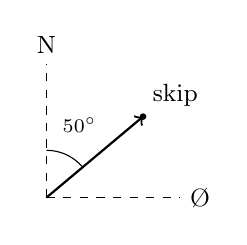
\begin{tikzpicture}[baseline=(current bounding box.north),font=\small]
  \draw[dashed] (0,0)--(0,1.7) node[above] {N};
  \draw[dashed] (0,0)--(1.7,0) node[right] {Ø};
  \draw[thick,->] (0,0)--(1.226,1.028);
  \draw (0,0.6) arc (90:40:0.6);
  \node[font=\scriptsize] at (0.42,0.92) {$50^\circ$};
  \fill (1.226,1.028) circle (1.2pt) node[above right] {skip};
\end{tikzpicture}
\end{minipage}\hfill
\begin{minipage}[t]{0.56\linewidth}
\textbf{Oppmåling fra to punkter.} Mål avstanden mellom punktene og vinkelen til målet fra hvert punkt.
\begin{enumerate}[leftmargin=1.4em,itemsep=1pt,topsep=2pt]
  \item Finn vinklene i den skjeve trekanten.
  \item Sinussetningen gir en skrå side.
  \item Sinus i den rettvinklede trekanten gir høyden.
\end{enumerate}
\textbf{Usikkerhet.} Endre vinkelen med $1^\circ$ og se hvor mye svaret endres.\par
\textbf{Avrunding.} Bruk lagrede verdier på kalkulatoren. Avrund til slutt.
\end{minipage}
\end{mustkunne}

\begin{eksempel}[1 — høyden av en mast]
\begin{minipage}[t]{0.52\linewidth}Fra $P$ er høydevinkelen til toppen av en mast $28^\circ$. Vi går $30$ m rett mot masten til $Q$. Der er høydevinkelen $41^\circ$. Finn høyden $h$. Svar med én desimal.
\end{minipage}\hfill
\begin{minipage}[t]{0.45\linewidth}
\centering
\begin{tikzpicture}[baseline=(current bounding box.north),font=\small,scale=0.9]
  \coordinate (P) at (0,0);
  \coordinate (Q) at (2.1,0);
  \coordinate (F) at (5.41,0);
  \coordinate (T) at (5.41,2.88);
  \draw[thick] (P)--(F);
  \draw[thick] (F)--(T) node[midway,right] {\color{niv3}\bfseries ?};
  \draw (P)--(T);
  \draw (Q)--(T);
  \draw (5.21,0)--(5.21,0.2)--(5.41,0.2);
  \draw (0.9,0) arc (0:28:0.9);
  \node[font=\scriptsize] at (1.25,0.17) {$28^\circ$};
  \draw (2.7,0) arc (0:41:0.6);
  \node[font=\scriptsize] at (3.1,0.25) {$41^\circ$};
  \draw[|-|] (0,-0.5)--(2.1,-0.5) node[midway,below] {\scriptsize$30$ m};
  \node[above] at (T) {$T$};
  \node[above left] at (P) {$P$};
  \node[above left] at (Q) {$Q$};
  \node[below] at (F) {$F$};
\end{tikzpicture}
\end{minipage}

\smallskip
\begin{stegtabell}
$\angle PQT = 180^\circ - 41^\circ = 139^\circ$ & Høydevinkelen $41^\circ$ er en ytre vinkel. Vinkelen i trekanten er $139^\circ$.\\
$\angle PTQ = 180^\circ - 28^\circ - 139^\circ = 13^\circ$ & Vinkelsum i trekant $PQT$.\\
$\dfrac{QT}{\sin 28^\circ} = \dfrac{30}{\sin 13^\circ}$ & Sinussetningen: $QT$ er overfor $28^\circ$, $PQ$ er overfor $13^\circ$.\\
$QT = \dfrac{30 \cdot \sin 28^\circ}{\sin 13^\circ} \approx 62,6$ m & Lagre verdien på kalkulatoren.\\
$h = QT \cdot \sin 41^\circ \approx 41,1$ m & Rettvinklet trekant $QFT$: motstående katet er hypotenus ganger sinus.\\
Kontroll: & $\frac{h}{\tan 28^\circ} - \frac{h}{\tan 41^\circ} = 77,3 - 47,3 = 30,0$, som er $PQ$.\\
\end{stegtabell}
\end{eksempel}

\begin{eksempel}[2 — navigasjon]
\begin{minipage}[t]{0.52\linewidth}En båt seiler fra $H$ kurs $40^\circ$ i $9$ km til $P$. Så seiler den kurs $100^\circ$ i $6$ km til $Q$. Finn avstanden $HQ$ og kursen fra $H$ rett til $Q$.
\end{minipage}\hfill
\begin{minipage}[t]{0.45\linewidth}
\centering
\begin{tikzpicture}[baseline=(current bounding box.north),font=\small,scale=1.2]
  \coordinate (H) at (0,0);
  \coordinate (P) at (50:2.25);
  \coordinate (Q) at ([shift={(-10:1.5)}]P);
  \draw[dashed] (H)--(0,1.2);
  \draw[dashed] (P)--([shift={(0,0.9)}]P);
  \draw[thick] (H)--(P) node[midway,above,sloped] {\scriptsize$9$ km};
  \draw[thick] (P)--(Q) node[midway,above,sloped] {\scriptsize$6$ km};
  \draw[thick,dashed] (H)--(Q) node[midway,below,sloped] {\color{niv3}\bfseries ?};
  \draw (0,0.5) arc (90:50:0.5);
  \node[font=\scriptsize] at (-0.3,0.7) {$40^\circ$};
  \draw ([shift={(0,0.35)}]P) arc (90:-10:0.35);
  \node[font=\scriptsize] at ([shift={(40:0.65)}]P) {$100^\circ$};
  \node[below left] at (H) {$H$};
  \node[left] at (P) {$P$};
  \node[right] at (Q) {$Q$};
\end{tikzpicture}
\end{minipage}

\smallskip
\begin{stegtabell}
$\angle HPQ = 180^\circ - (100^\circ - 40^\circ) = 120^\circ$ & Båten svinger $60^\circ$ til høyre. Vinkelen inne i trekanten er $180^\circ - 60^\circ$.\\
$HQ^2 = 9^2 + 6^2 - 2 \cdot 9 \cdot 6 \cdot \cos 120^\circ = 171$ & To sider og vinkelen mellom: cosinussetningen.\\
$HQ = \sqrt{171} \approx 13,1$ km & Kvadratrot til slutt.\\
$\sin H = \dfrac{6 \cdot \sin 120^\circ}{HQ}$, så $H \approx 23,4^\circ$ & Sinussetningen. $PQ$ er korteste side, så $H$ er spiss.\\
kurs $= 40^\circ + 23,4^\circ = 63,4^\circ$ & $Q$ ligger til høyre for linja $HP$. Da legger vi vinkelen til kursen.\\
\end{stegtabell}
\end{eksempel}

\begin{vanligfeil}
\begin{itemize}[leftmargin=1.2em,itemsep=1pt,topsep=0pt]
  \item Du tegner kurs $40^\circ$ som $40^\circ$ fra $x$-aksen. Det er feil. Kurs måles fra nord med klokka, så kurs $40^\circ$ er $90^\circ - 40^\circ = 50^\circ$ fra øst-aksen.
  \item Du bruker høydevinkelen $41^\circ$ som vinkel inni trekanten $PQT$. Det er feil. Vinkelen i trekanten er $180^\circ - 41^\circ = 139^\circ$.
  \item Du avrunder underveis. Rundes sinusverdiene i eksempel 1 til to desimaler, blir svaret ca. $42,3$ m i stedet for $41,1$ m.
\end{itemize}
\end{vanligfeil}

\nivaahode{1}

\oppg{2.1}{1}{\mh}
Et skip seiler kurs $70^\circ$. Tegn en skisse med nord opp.
\begin{tasks}(1)
  \task Hvilken av retningene nord, øst, sør og vest ligger kursen nærmest?
  \task Hvilken kurs har skipet hvis det snur og seiler rett tilbake?
  \task Skipet svinger til kurs $150^\circ$. Hvor mange grader har det svingt?
\end{tasks}

\oppg{2.2}{1}{\mh}
Du står $45$ m fra foten av en flaggstang på flatt terreng. Høydevinkelen til toppen er $32^\circ$. Hvor høy er flaggstanga? Se bort fra øyehøyden. Svar med én desimal.

\oppg{2.3}{1}{\mh}
To båter $A$ og $B$ ligger $200$ m fra hverandre. Begge sikter mot en bøye $C$. I trekant $ABC$ er $\angle A = 50^\circ$ og $\angle B = 64^\circ$. Tegn en skisse og fullfør.
\begin{tasks}(1)
  \task $\angle C = 180^\circ - 50^\circ - 64^\circ = \skrivlinje[15mm]$.
  \task $\dfrac{AC}{\sin 64^\circ} = \dfrac{200}{\sin\skrivlinje[12mm]}$, så $AC \approx \skrivlinje[2cm]$ m.
  \task Finn $BC$ på samme måte.
\end{tasks}

\nivaahode{2}

\oppg{2.4}{2}{\mh}
\begin{minipage}[t]{0.50\linewidth}
Fra to punkter $A$ og $B$ på samme elvebredd, $75$ m fra hverandre, ser vi et tre $T$ på motsatt bredd. Vi måler $\angle TAB = 58^\circ$ og $\angle TBA = 74^\circ$. Finn bredden av elva, altså korteste avstand fra $T$ til linja $AB$. Svar med én desimal.
\end{minipage}\hfill
\begin{minipage}[t]{0.47\linewidth}
\centering
\begin{tikzpicture}[baseline=(current bounding box.north),font=\small,scale=0.9]
  \fill[blue!10] (-0.5,0) rectangle (3.5,3.29);
  \draw (-0.5,0)--(3.5,0);
  \draw (-0.5,3.29)--(3.5,3.29);
  \coordinate (A) at (0,0);
  \coordinate (B) at (3,0);
  \coordinate (T) at (2.056,3.29);
  \coordinate (F) at (2.056,0);
  \draw[thick] (A)--(T)--(B);
  \draw[dashed] (T)--(F) node[midway,left] {\color{niv3}\bfseries ?};
  \draw (1.856,0)--(1.856,0.2)--(2.056,0.2);
  \draw (0.7,0) arc (0:58:0.7);
  \node[font=\scriptsize] at (1.0,0.3) {$58^\circ$};
  \draw (2.4,0) arc (180:106:0.6);
  \node[font=\scriptsize] at (2.28,0.45) {$74^\circ$};
  \draw[|-|] (0,-0.5)--(3,-0.5) node[midway,below] {\scriptsize$75$ m};
  \node[left] at (A) {$A$};
  \node[right] at (B) {$B$};
  \node[above] at (T) {$T$};
\end{tikzpicture}
\end{minipage}

\oppg{2.5}{2}{\mh}
En båt seiler fra $H$ kurs $30^\circ$ i $15$ km til $P$. Så seiler den kurs $160^\circ$ i $10$ km til $Q$. Tegn en skisse.
\begin{tasks}(2)
  \task Finn $\angle HPQ$.
  \task Finn avstanden $HQ$.
  \task Finn $\angle PHQ$.
  \task Hvilken kurs må båten ha fra $Q$ for å seile rett tilbake til $H$?
\end{tasks}

\oppg{2.6}{2}{\mh}
Fra $A$ er høydevinkelen til toppen $T$ av et fjell $20^\circ$. Vi går $300$ m rett mot fjellet til $B$. Der er høydevinkelen $32^\circ$. Eleven skal finne høyden $h$ av fjelltoppen over bakken. Finn \textbf{den første feilen}. Løs riktig.
\[ \begin{aligned}
\angle ATB &= 32^\circ - 20^\circ = 12^\circ\\
\angle ABT &= 180^\circ - 32^\circ = 148^\circ\\
BT &= \frac{300 \cdot \sin 20^\circ}{\sin 12^\circ} \approx 493,5 \text{ m}\\
h &= BT \cdot \sin 20^\circ \approx 168,8 \text{ m}
\end{aligned} \]

\oppg{2.7}{2}{\mh}
\begin{minipage}[t]{0.46\linewidth}
Et tak har bredde $10$ m. De to takflatene har vinklene $35^\circ$ og $50^\circ$ mot vannrett. Finn lengden av begge sperrene og mønehøyden, altså høyden fra mønet ned til bakken. Svar med én desimal.
\end{minipage}\hfill
\begin{minipage}[t]{0.50\linewidth}
\centering
\begin{tikzpicture}[baseline=(current bounding box.north),font=\small,scale=0.8]
  \coordinate (A) at (0,0);
  \coordinate (B) at (7,0);
  \coordinate (C) at (4.41,3.087);
  \coordinate (F) at (4.41,0);
  \draw[thick] (A)--(B);
  \draw[thick] (A)--(C) node[midway,above,sloped] {\color{niv3}\bfseries ?};
  \draw[thick] (C)--(B) node[midway,above,sloped] {\color{niv3}\bfseries ?};
  \draw[dashed] (C)--(F) node[midway,left] {\color{niv3}\bfseries ?};
  \draw (4.21,0)--(4.21,0.2)--(4.41,0.2);
  \draw (1,0) arc (0:35:1);
  \node[font=\scriptsize] at (1.4,0.2) {$35^\circ$};
  \draw (6,0) arc (180:130:1);
  \node[font=\scriptsize] at (5.55,0.2) {$50^\circ$};
  \draw[|-|] (0,-0.5)--(7,-0.5) node[midway,below] {\scriptsize$10$ m};
  \node[left] at (A) {$A$};
  \node[right] at (B) {$B$};
  \node[above] at (C) {$C$};
\end{tikzpicture}
\end{minipage}

\nivaahode{3}

\oppg{2.8}{3}{\mh}
En landmåler står $80$ m fra foten av en mast på flatt terreng og måler høydevinkelen til toppen med usikkerhet $\pm 1^\circ$.
\begin{tasks}(1)
  \task Vinkelen er $25^\circ$. Finn høyden når vinkelen er $25^\circ$, og den minste og største mulige høyden.
  \task En annen mast, like langt unna, har høydevinkel $60^\circ$. Gjør det samme.
  \task Forklar hvorfor usikkerheten i meter blir større i b) enn i a).
\end{tasks}

\oppg{2.9}{3}{\mh}
To skip forlater en havn samtidig. Skip $A$ seiler kurs $30^\circ$ med fart $30$ km/t. Skip $B$ seiler kurs $90^\circ$. Etter $2$ timer er avstanden mellom skipene $52$ km.
\begin{tasks}(1)
  \task Tegn en skisse. Finn vinkelen mellom de to kursene.
  \task Finn farten til skip $B$. Er det mer enn ett mulig svar?
  \task Forklar hvorfor oppgaven har det antallet svar.
\end{tasks}

\begin{sjekk}
\begin{tasks}(2)
  \task Et skip seiler kurs $310^\circ$. Hvilken kurs har det rett tilbake?
  \task Du står $30$ m fra et hus. Høydevinkelen til taket er $45^\circ$. Hvor høyt er huset?
  \task! Hvorfor lagrer vi mellomsvar på kalkulatoren og avrunder bare til slutt?
\end{tasks}
\end{sjekk}
